 \documentclass [12pt]{article} 

\usepackage {amsmath}
\usepackage {amsthm}
\usepackage {amssymb}
\usepackage {graphicx} 
\usepackage {float}
\usepackage {multirow}
\usepackage {xcolor}
\usepackage {algorithmic}
\usepackage [ruled,vlined,commentsnumbered,titlenotnumbered]{algorithm2e} \usepackage {array} 
\usepackage {booktabs} 
\usepackage {url} 
\usepackage {parskip} 
\usepackage [margin=1in]{geometry} 
\usepackage [T1]{fontenc} 
\usepackage {cmbright} 
\usepackage [many]{tcolorbox} 
\usepackage [colorlinks = true,
            linkcolor = blue,
            urlcolor  = blue,
            citecolor = blue,
            anchorcolor = blue]{hyperref} 
\usepackage {enumitem} 
\usepackage {xparse} 
\usepackage {verbatim}
\usepackage{listings}
\usepackage{xcolor}
\lstset { %
    language=C++,
    backgroundcolor=\color{black!5}, % set backgroundcolor
    basicstyle=\footnotesize,% basic font setting
}
\newtheorem{theorem}{Theorem}
\newtheorem{remark}{Remark}



\DeclareTColorBox {Solution}{}{breakable, title={Solution}} \DeclareTColorBox {Solution*}{}{breakable, title={Solution (provided)}} \DeclareTColorBox {Instruction}{}{boxrule=0pt, boxsep=0pt, left=0.5em, right=0.5em, top=0.5em, bottom=0.5em, arc=0pt, toprule=1pt, bottomrule=1pt} \DeclareDocumentCommand {\Expecting }{+m}{\textbf {[We are expecting:} #1\textbf {]}} \DeclareDocumentCommand {\Points }{m}{\textbf {(#1 pt.)}} 

\begin {document} 

\vspace {1em} 
\begin {Instruction} 
Adapted From Virginia Williams' lecture notes.
\end {Instruction}  

{\LARGE \textbf {COMP 285 (NC A\&T, Spr `22)}\hfill \textbf {Lecture 16} } 

\begin{centering}
\section{Breadth-First Search}
 
 In depth first search, we search ``deeper'' in the graph whenever possible, exploring edges out of the most recently discovered node that still has unexplored edges leaving it. Breadth first search (BFS) instead expands the frontier between discovered and undiscovered nodes uniformly across the breadth of the frontier, discovering all nodes at a distance $k$ from the source node before nodes at distance $k + 1$. BFS($s$) computes for every node $v \in G$ the distance from $s$ to $v$ in $G$. $d(u, v )$ is the length of the shortest path from $u$ to $v$ . A simple property of unweighted graphs is as follows: let $P$ be a shortest $u \to v$ path and let $x$ be the node before $v$ on $P$. Then $d(u, v) = d(u, x) + 1$.


\begin{center}
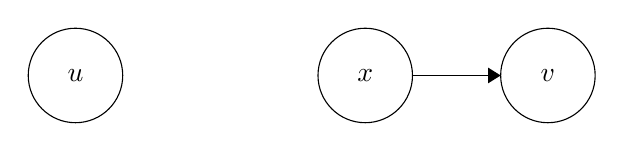
\begin{tikzpicture}[scale=0.2]
\tikzstyle{every node}+=[inner sep=0pt]
\draw [black] (22.9,-24.5) circle (3);
\draw (22.9,-24.5) node {$u$};
\draw [black] (41.3,-24.5) circle (3);
\draw (41.3,-24.5) node {$x$};
\draw [black] (52.9,-24.5) circle (3);
\draw (52.9,-24.5) node {$v$};
\draw [black] (44.3,-24.5) -- (49.9,-24.5);
\fill [black] (49.9,-24.5) -- (49.1,-24) -- (49.1,-25);
\end{tikzpicture}
\end{center}


\end{centering}







\end{document}